\documentclass[1p]{elsarticle_modified}
%\bibliographystyle{elsarticle-num}

%\usepackage[colorlinks]{hyperref}
%\usepackage{abbrmath_seonhwa} %\Abb, \Ascr, \Acal ,\Abf, \Afrak
\usepackage{amsfonts}
\usepackage{amssymb}
\usepackage{amsmath}
\usepackage{amsthm}
\usepackage{scalefnt}
\usepackage{amsbsy}
\usepackage{kotex}
\usepackage{caption}
\usepackage{subfig}
\usepackage{color}
\usepackage{graphicx}
\usepackage{xcolor} %% white, black, red, green, blue, cyan, magenta, yellow
\usepackage{float}
\usepackage{setspace}
\usepackage{hyperref}

\usepackage{tikz}
\usetikzlibrary{arrows}

\usepackage{multirow}
\usepackage{array} % fixed length table
\usepackage{hhline}

%%%%%%%%%%%%%%%%%%%%%
\makeatletter
\renewcommand*\env@matrix[1][\arraystretch]{%
	\edef\arraystretch{#1}%
	\hskip -\arraycolsep
	\let\@ifnextchar\new@ifnextchar
	\array{*\c@MaxMatrixCols c}}
\makeatother %https://tex.stackexchange.com/questions/14071/how-can-i-increase-the-line-spacing-in-a-matrix
%%%%%%%%%%%%%%%

\usepackage[normalem]{ulem}

\newcommand{\msout}[1]{\ifmmode\text{\sout{\ensuremath{#1}}}\else\sout{#1}\fi}
%SOURCE: \msout is \stkout macro in https://tex.stackexchange.com/questions/20609/strikeout-in-math-mode

\newcommand{\cancel}[1]{
	\ifmmode
	{\color{red}\msout{#1}}
	\else
	{\color{red}\sout{#1}}
	\fi
}

\newcommand{\add}[1]{
	{\color{blue}\uwave{#1}}
}

\newcommand{\replace}[2]{
	\ifmmode
	{\color{red}\msout{#1}}{\color{blue}\uwave{#2}}
	\else
	{\color{red}\sout{#1}}{\color{blue}\uwave{#2}}
	\fi
}

\newcommand{\Sol}{\mathcal{S}} %segment
\newcommand{\D}{D} %diagram
\newcommand{\A}{\mathcal{A}} %arc


%%%%%%%%%%%%%%%%%%%%%%%%%%%%%5 test

\def\sl{\operatorname{\textup{SL}}(2,\Cbb)}
\def\psl{\operatorname{\textup{PSL}}(2,\Cbb)}
\def\quan{\mkern 1mu \triangleright \mkern 1mu}

\theoremstyle{definition}
\newtheorem{thm}{Theorem}[section]
\newtheorem{prop}[thm]{Proposition}
\newtheorem{lem}[thm]{Lemma}
\newtheorem{ques}[thm]{Question}
\newtheorem{cor}[thm]{Corollary}
\newtheorem{defn}[thm]{Definition}
\newtheorem{exam}[thm]{Example}
\newtheorem{rmk}[thm]{Remark}
\newtheorem{alg}[thm]{Algorithm}

\newcommand{\I}{\sqrt{-1}}
\begin{document}

%\begin{frontmatter}
%
%\title{Boundary parabolic representations of knots up to 8 crossings}
%
%%% Group authors per affiliation:
%\author{Yunhi Cho} 
%\address{Department of Mathematics, University of Seoul, Seoul, Korea}
%\ead{yhcho@uos.ac.kr}
%
%
%\author{Seonhwa Kim} %\fnref{s_kim}}
%\address{Center for Geometry and Physics, Institute for Basic Science, Pohang, 37673, Korea}
%\ead{ryeona17@ibs.re.kr}
%
%\author{Hyuk Kim}
%\address{Department of Mathematical Sciences, Seoul National University, Seoul 08826, Korea}
%\ead{hyukkim@snu.ac.kr}
%
%\author{Seokbeom Yoon}
%\address{Department of Mathematical Sciences, Seoul National University, Seoul, 08826,  Korea}
%\ead{sbyoon15@snu.ac.kr}
%
%\begin{abstract}
%We find all boundary parabolic representation of knots up to 8 crossings.
%
%\end{abstract}
%\begin{keyword}
%    \MSC[2010] 57M25 
%\end{keyword}
%
%\end{frontmatter}

%\linenumbers
%\tableofcontents
%
\newcommand\colored[1]{\textcolor{white}{\rule[-0.35ex]{0.8em}{1.4ex}}\kern-0.8em\color{red} #1}%
%\newcommand\colored[1]{\textcolor{white}{ #1}\kern-2.17ex	\textcolor{white}{ #1}\kern-1.81ex	\textcolor{white}{ #1}\kern-2.15ex\color{red}#1	}

{\Large $\underline{12n_{0516}~(K12n_{0516})}$}

\setlength{\tabcolsep}{10pt}
\renewcommand{\arraystretch}{1.6}
\vspace{1cm}\begin{tabular}{m{100pt}>{\centering\arraybackslash}m{274pt}}
\multirow{5}{120pt}{
	\centering
	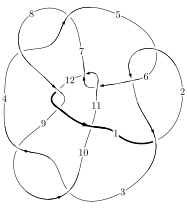
\includegraphics[width=112pt]{../../../GIT/diagram.site/Diagrams/png/2605_12n_0516.png}\\
\ \ \ A knot diagram\footnotemark}&
\allowdisplaybreaks
\textbf{Linearized knot diagam} \\
\cline{2-2}
 &
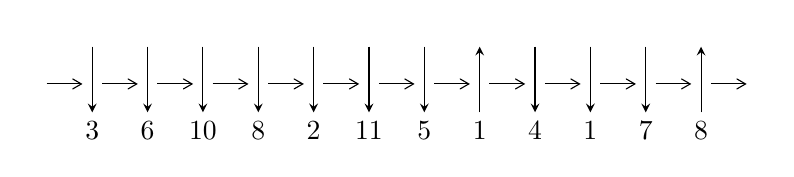
\begin{tikzpicture}[x=20pt, y=17pt]
	% nodes
	\node (C0) at (0, 0) {};
	\node (C1) at (1, 0) {};
	\node (C1U) at (1, +1) {};
	\node (C1D) at (1, -1) {3};

	\node (C2) at (2, 0) {};
	\node (C2U) at (2, +1) {};
	\node (C2D) at (2, -1) {6};

	\node (C3) at (3, 0) {};
	\node (C3U) at (3, +1) {};
	\node (C3D) at (3, -1) {10};

	\node (C4) at (4, 0) {};
	\node (C4U) at (4, +1) {};
	\node (C4D) at (4, -1) {8};

	\node (C5) at (5, 0) {};
	\node (C5U) at (5, +1) {};
	\node (C5D) at (5, -1) {2};

	\node (C6) at (6, 0) {};
	\node (C6U) at (6, +1) {};
	\node (C6D) at (6, -1) {11};

	\node (C7) at (7, 0) {};
	\node (C7U) at (7, +1) {};
	\node (C7D) at (7, -1) {5};

	\node (C8) at (8, 0) {};
	\node (C8U) at (8, +1) {};
	\node (C8D) at (8, -1) {1};

	\node (C9) at (9, 0) {};
	\node (C9U) at (9, +1) {};
	\node (C9D) at (9, -1) {4};

	\node (C10) at (10, 0) {};
	\node (C10U) at (10, +1) {};
	\node (C10D) at (10, -1) {1};

	\node (C11) at (11, 0) {};
	\node (C11U) at (11, +1) {};
	\node (C11D) at (11, -1) {7};

	\node (C12) at (12, 0) {};
	\node (C12U) at (12, +1) {};
	\node (C12D) at (12, -1) {8};
	\node (C13) at (13, 0) {};

	% arrows
	\draw[->,>={angle 60}]
	(C0) edge (C1) (C1) edge (C2) (C2) edge (C3) (C3) edge (C4) (C4) edge (C5) (C5) edge (C6) (C6) edge (C7) (C7) edge (C8) (C8) edge (C9) (C9) edge (C10) (C10) edge (C11) (C11) edge (C12) (C12) edge (C13) ;	\draw[->,>=stealth]
	(C1U) edge (C1D) (C2U) edge (C2D) (C3U) edge (C3D) (C4U) edge (C4D) (C5U) edge (C5D) (C6U) edge (C6D) (C7U) edge (C7D) (C8D) edge (C8U) (C9U) edge (C9D) (C10U) edge (C10D) (C11U) edge (C11D) (C12D) edge (C12U) ;
	\end{tikzpicture} \\
\hhline{~~} \\& 
\textbf{Solving Sequence} \\ \cline{2-2} 
 &
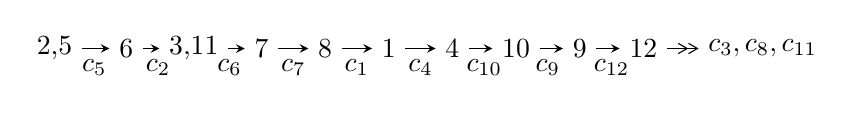
\begin{tikzpicture}[x=23pt, y=7pt]
	% node
	\node (A0) at (-1/8, 0) {2,5};
	\node (A1) at (1, 0) {6};
	\node (A2) at (33/16, 0) {3,11};
	\node (A3) at (25/8, 0) {7};
	\node (A4) at (33/8, 0) {8};
	\node (A5) at (41/8, 0) {1};
	\node (A6) at (49/8, 0) {4};
	\node (A7) at (57/8, 0) {10};
	\node (A8) at (65/8, 0) {9};
	\node (A9) at (73/8, 0) {12};
	\node (C1) at (1/2, -1) {$c_{5}$};
	\node (C2) at (3/2, -1) {$c_{2}$};
	\node (C3) at (21/8, -1) {$c_{6}$};
	\node (C4) at (29/8, -1) {$c_{7}$};
	\node (C5) at (37/8, -1) {$c_{1}$};
	\node (C6) at (45/8, -1) {$c_{4}$};
	\node (C7) at (53/8, -1) {$c_{10}$};
	\node (C8) at (61/8, -1) {$c_{9}$};
	\node (C9) at (69/8, -1) {$c_{12}$};
	\node (A10) at (11, 0) {$c_{3},c_{8},c_{11}$};

	% edge
	\draw[->,>=stealth]	
	(A0) edge (A1) (A1) edge (A2) (A2) edge (A3) (A3) edge (A4) (A4) edge (A5) (A5) edge (A6) (A6) edge (A7) (A7) edge (A8) (A8) edge (A9) ;
	\draw[->>,>={angle 60}]	
	(A9) edge (A10);
\end{tikzpicture} \\ 

\end{tabular} \\

\footnotetext{
The image of knot diagram is generated by the software ``\textbf{Draw programme}" developed by Andrew Bartholomew(\url{http://www.layer8.co.uk/maths/draw/index.htm\#Running-draw}), where we modified some parts for our purpose(\url{https://github.com/CATsTAILs/LinksPainter}).
}\phantom \\ \newline 
\centering \textbf{Ideals for irreducible components\footnotemark of $X_{\text{par}}$} 
 
\begin{align*}
I^u_{1}&=\langle 
-7.85298\times10^{46} u^{63}-5.20735\times10^{47} u^{62}+\cdots+6.20841\times10^{47} b-2.06005\times10^{48},\\
\phantom{I^u_{1}}&\phantom{= \langle  }-7.35896\times10^{48} u^{63}-9.51515\times10^{48} u^{62}+\cdots+4.34588\times10^{48} a+4.04153\times10^{49},\;u^{64}+u^{63}+\cdots+u-7\rangle \\
I^u_{2}&=\langle 
u^{13}-2 u^{11}+u^{10}+5 u^9- u^8-6 u^7+3 u^6+6 u^5-2 u^4-3 u^3+2 u^2+b+u-1,\;- u^{15}+2 u^{14}+\cdots+a-3,\\
\phantom{I^u_{2}}&\phantom{= \langle  }u^{16}-3 u^{14}+u^{13}+8 u^{12}-2 u^{11}-13 u^{10}+5 u^9+17 u^8-6 u^7-15 u^6+6 u^5+10 u^4-4 u^3-4 u^2+u+1\rangle \\
\\
\end{align*}
\raggedright * 2 irreducible components of $\dim_{\mathbb{C}}=0$, with total 80 representations.\\
\footnotetext{All coefficients of polynomials are rational numbers. But the coefficients are sometimes approximated in decimal forms when there is not enough margin.}
\newpage
\renewcommand{\arraystretch}{1}
\centering \section*{I. $I^u_{1}= \langle -7.85\times10^{46} u^{63}-5.21\times10^{47} u^{62}+\cdots+6.21\times10^{47} b-2.06\times10^{48},\;-7.36\times10^{48} u^{63}-9.52\times10^{48} u^{62}+\cdots+4.35\times10^{48} a+4.04\times10^{49},\;u^{64}+u^{63}+\cdots+u-7 \rangle$}
\flushleft \textbf{(i) Arc colorings}\\
\begin{tabular}{m{7pt} m{180pt} m{7pt} m{180pt} }
\flushright $a_{2}=$&$\begin{pmatrix}0\\u\end{pmatrix}$ \\
\flushright $a_{5}=$&$\begin{pmatrix}1\\0\end{pmatrix}$ \\
\flushright $a_{6}=$&$\begin{pmatrix}1\\u^2\end{pmatrix}$ \\
\flushright $a_{3}=$&$\begin{pmatrix}- u\\- u^3+u\end{pmatrix}$ \\
\flushright $a_{11}=$&$\begin{pmatrix}1.69332 u^{63}+2.18946 u^{62}+\cdots-1.36290 u-9.29967\\0.126489 u^{63}+0.838758 u^{62}+\cdots+0.322847 u+3.31817\end{pmatrix}$ \\
\flushright $a_{7}=$&$\begin{pmatrix}0.458095 u^{63}+0.270972 u^{62}+\cdots+5.77781 u-3.68320\\-0.652252 u^{63}-0.459949 u^{62}+\cdots-3.70273 u-0.960278\end{pmatrix}$ \\
\flushright $a_{8}=$&$\begin{pmatrix}1.11035 u^{63}+0.730921 u^{62}+\cdots+9.48054 u-2.72293\\-0.652252 u^{63}-0.459949 u^{62}+\cdots-3.70273 u-0.960278\end{pmatrix}$ \\
\flushright $a_{1}=$&$\begin{pmatrix}u^3\\u^5- u^3+u\end{pmatrix}$ \\
\flushright $a_{4}=$&$\begin{pmatrix}-0.390009 u^{63}+1.20156 u^{62}+\cdots+9.75516 u+2.37373\\-1.02634 u^{63}-2.06653 u^{62}+\cdots-6.84016 u+0.604319\end{pmatrix}$ \\
\flushright $a_{10}=$&$\begin{pmatrix}1.03280 u^{63}+0.937261 u^{62}+\cdots-5.99095 u-13.2305\\0.117302 u^{63}+0.462797 u^{62}+\cdots+0.960616 u+2.35400\end{pmatrix}$ \\
\flushright $a_{9}=$&$\begin{pmatrix}-1.98871 u^{63}-1.59326 u^{62}+\cdots-13.0023 u+2.89409\\0.669965 u^{63}+0.133677 u^{62}+\cdots+3.58629 u-0.901368\end{pmatrix}$ \\
\flushright $a_{12}=$&$\begin{pmatrix}0.547710 u^{63}+1.84010 u^{62}+\cdots-2.73316 u+10.4198\\1.08225 u^{63}+0.435476 u^{62}+\cdots+6.51395 u+1.98262\end{pmatrix}$\\&\end{tabular}
\flushleft \textbf{(ii) Obstruction class $= -1$}\\~\\
\flushleft \textbf{(iii) Cusp Shapes $= -3.58831 u^{63}-4.70243 u^{62}+\cdots-11.8066 u-39.5814$}\\~\\
\newpage\renewcommand{\arraystretch}{1}
\flushleft \textbf{(iv) u-Polynomials at the component}\newline \\
\begin{tabular}{m{50pt}|m{274pt}}
Crossings & \hspace{64pt}u-Polynomials at each crossing \\
\hline $$\begin{aligned}c_{1}\end{aligned}$$&$\begin{aligned}
&u^{64}+25 u^{63}+\cdots+365 u+49
\end{aligned}$\\
\hline $$\begin{aligned}c_{2},c_{5}\end{aligned}$$&$\begin{aligned}
&u^{64}+u^{63}+\cdots+u-7
\end{aligned}$\\
\hline $$\begin{aligned}c_{3},c_{9}\end{aligned}$$&$\begin{aligned}
&u^{64}+u^{63}+\cdots-21 u-11
\end{aligned}$\\
\hline $$\begin{aligned}c_{4},c_{7}\end{aligned}$$&$\begin{aligned}
&u^{64}-3 u^{63}+\cdots+9 u-1
\end{aligned}$\\
\hline $$\begin{aligned}c_{6},c_{11}\end{aligned}$$&$\begin{aligned}
&u^{64}-3 u^{63}+\cdots-2134 u+163
\end{aligned}$\\
\hline $$\begin{aligned}c_{8},c_{12}\end{aligned}$$&$\begin{aligned}
&u^{64}+3 u^{63}+\cdots-44 u+1
\end{aligned}$\\
\hline $$\begin{aligned}c_{10}\end{aligned}$$&$\begin{aligned}
&u^{64}+u^{63}+\cdots+1218 u+817
\end{aligned}$\\
\hline
\end{tabular}\\~\\
\newpage\renewcommand{\arraystretch}{1}
\flushleft \textbf{(v) Riley Polynomials at the component}\newline \\
\begin{tabular}{m{50pt}|m{274pt}}
Crossings & \hspace{64pt}Riley Polynomials at each crossing \\
\hline $$\begin{aligned}c_{1}\end{aligned}$$&$\begin{aligned}
&y^{64}+35 y^{63}+\cdots-129697 y+2401
\end{aligned}$\\
\hline $$\begin{aligned}c_{2},c_{5}\end{aligned}$$&$\begin{aligned}
&y^{64}-25 y^{63}+\cdots-365 y+49
\end{aligned}$\\
\hline $$\begin{aligned}c_{3},c_{9}\end{aligned}$$&$\begin{aligned}
&y^{64}+21 y^{63}+\cdots+1847 y+121
\end{aligned}$\\
\hline $$\begin{aligned}c_{4},c_{7}\end{aligned}$$&$\begin{aligned}
&y^{64}+3 y^{63}+\cdots+67 y+1
\end{aligned}$\\
\hline $$\begin{aligned}c_{6},c_{11}\end{aligned}$$&$\begin{aligned}
&y^{64}-51 y^{63}+\cdots-1941718 y+26569
\end{aligned}$\\
\hline $$\begin{aligned}c_{8},c_{12}\end{aligned}$$&$\begin{aligned}
&y^{64}+63 y^{63}+\cdots-222 y+1
\end{aligned}$\\
\hline $$\begin{aligned}c_{10}\end{aligned}$$&$\begin{aligned}
&y^{64}-17 y^{63}+\cdots-71533104 y+667489
\end{aligned}$\\
\hline
\end{tabular}\\~\\
\newpage\flushleft \textbf{(vi) Complex Volumes and Cusp Shapes}
$$\begin{array}{c|c|c}  
\text{Solutions to }I^u_{1}& \I (\text{vol} + \sqrt{-1}CS) & \text{Cusp shape}\\
 \hline 
\begin{aligned}
u &= -0.371115 + 0.915968 I \\
a &= -0.249549 + 0.000216 I \\
b &= \phantom{-}1.41996 - 0.06852 I\end{aligned}
 & -4.48635 + 5.15157 I & -8.61815 - 5.07687 I \\ \hline\begin{aligned}
u &= -0.371115 - 0.915968 I \\
a &= -0.249549 - 0.000216 I \\
b &= \phantom{-}1.41996 + 0.06852 I\end{aligned}
 & -4.48635 - 5.15157 I & -8.61815 + 5.07687 I \\ \hline\begin{aligned}
u &= -0.857881 + 0.542275 I \\
a &= -1.74491 - 1.24280 I \\
b &= -0.157463 + 1.230750 I\end{aligned}
 & \phantom{-}3.16250 + 2.17822 I & -8.00000 - 2.65918 I \\ \hline\begin{aligned}
u &= -0.857881 - 0.542275 I \\
a &= -1.74491 + 1.24280 I \\
b &= -0.157463 - 1.230750 I\end{aligned}
 & \phantom{-}3.16250 - 2.17822 I & -8.00000 + 2.65918 I \\ \hline\begin{aligned}
u &= -0.774165 + 0.604979 I \\
a &= -0.379187 - 0.211028 I \\
b &= -1.184290 - 0.467280 I\end{aligned}
 & -0.067270 - 0.618429 I & -7.06284 - 1.08548 I \\ \hline\begin{aligned}
u &= -0.774165 - 0.604979 I \\
a &= -0.379187 + 0.211028 I \\
b &= -1.184290 + 0.467280 I\end{aligned}
 & -0.067270 + 0.618429 I & -7.06284 + 1.08548 I \\ \hline\begin{aligned}
u &= -0.697346 + 0.673163 I \\
a &= -1.356820 - 0.219530 I \\
b &= -0.281088 - 0.295837 I\end{aligned}
 & \phantom{-}1.16285 - 2.77092 I & -3.07563 + 5.25924 I \\ \hline\begin{aligned}
u &= -0.697346 - 0.673163 I \\
a &= -1.356820 + 0.219530 I \\
b &= -0.281088 + 0.295837 I\end{aligned}
 & \phantom{-}1.16285 + 2.77092 I & -3.07563 - 5.25924 I \\ \hline\begin{aligned}
u &= -0.650023 + 0.706094 I \\
a &= -0.285329 + 0.030490 I \\
b &= -1.046050 - 0.338958 I\end{aligned}
 & -0.317206 - 0.693581 I & -9.74422 - 0.91005 I \\ \hline\begin{aligned}
u &= -0.650023 - 0.706094 I \\
a &= -0.285329 - 0.030490 I \\
b &= -1.046050 + 0.338958 I\end{aligned}
 & -0.317206 + 0.693581 I & -9.74422 + 0.91005 I\\
 \hline 
 \end{array}$$\newpage$$\begin{array}{c|c|c}  
\text{Solutions to }I^u_{1}& \I (\text{vol} + \sqrt{-1}CS) & \text{Cusp shape}\\
 \hline 
\begin{aligned}
u &= -1.005520 + 0.304620 I \\
a &= -0.923017 + 0.876033 I \\
b &= -0.04591 + 1.48528 I\end{aligned}
 & -3.50871 + 0.31411 I & -14.0279 - 2.5519 I \\ \hline\begin{aligned}
u &= -1.005520 - 0.304620 I \\
a &= -0.923017 - 0.876033 I \\
b &= -0.04591 - 1.48528 I\end{aligned}
 & -3.50871 - 0.31411 I & -14.0279 + 2.5519 I \\ \hline\begin{aligned}
u &= \phantom{-}1.06514\phantom{ +0.000000I} \\
a &= \phantom{-}2.45909\phantom{ +0.000000I} \\
b &= \phantom{-}1.23942\phantom{ +0.000000I}\end{aligned}
 & -5.55858\phantom{ +0.000000I} & -18.6480\phantom{ +0.000000I} \\ \hline\begin{aligned}
u &= -0.895727 + 0.581855 I \\
a &= \phantom{-}1.75893 + 1.76078 I \\
b &= \phantom{-}1.60878 - 0.32014 I\end{aligned}
 & -0.42753 + 5.30671 I & -8.00000 - 5.96802 I \\ \hline\begin{aligned}
u &= -0.895727 - 0.581855 I \\
a &= \phantom{-}1.75893 - 1.76078 I \\
b &= \phantom{-}1.60878 + 0.32014 I\end{aligned}
 & -0.42753 - 5.30671 I & -8.00000 + 5.96802 I \\ \hline\begin{aligned}
u &= \phantom{-}0.597067 + 0.892023 I \\
a &= \phantom{-}0.024569 + 0.245452 I \\
b &= -1.45388 - 0.06677 I\end{aligned}
 & -3.48226 + 1.14380 I & \phantom{-0.000000 } 0 \\ \hline\begin{aligned}
u &= \phantom{-}0.597067 - 0.892023 I \\
a &= \phantom{-}0.024569 - 0.245452 I \\
b &= -1.45388 + 0.06677 I\end{aligned}
 & -3.48226 - 1.14380 I & \phantom{-0.000000 } 0 \\ \hline\begin{aligned}
u &= -0.559478 + 0.919447 I \\
a &= -0.206651 - 0.005295 I \\
b &= \phantom{-}1.53912 + 0.83354 I\end{aligned}
 & -3.36566 - 9.85168 I & \phantom{-0.000000 } 0 \\ \hline\begin{aligned}
u &= -0.559478 - 0.919447 I \\
a &= -0.206651 + 0.005295 I \\
b &= \phantom{-}1.53912 - 0.83354 I\end{aligned}
 & -3.36566 + 9.85168 I & \phantom{-0.000000 } 0 \\ \hline\begin{aligned}
u &= \phantom{-}0.916404 + 0.593398 I \\
a &= \phantom{-}0.319890 + 0.450880 I \\
b &= \phantom{-}0.167272 - 0.326682 I\end{aligned}
 & \phantom{-}1.79208 - 3.22792 I & \phantom{-0.000000 } 0\\
 \hline 
 \end{array}$$\newpage$$\begin{array}{c|c|c}  
\text{Solutions to }I^u_{1}& \I (\text{vol} + \sqrt{-1}CS) & \text{Cusp shape}\\
 \hline 
\begin{aligned}
u &= \phantom{-}0.916404 - 0.593398 I \\
a &= \phantom{-}0.319890 - 0.450880 I \\
b &= \phantom{-}0.167272 + 0.326682 I\end{aligned}
 & \phantom{-}1.79208 + 3.22792 I & \phantom{-0.000000 } 0 \\ \hline\begin{aligned}
u &= \phantom{-}0.968315 + 0.512599 I \\
a &= \phantom{-}0.667248 + 1.104970 I \\
b &= -1.13705 + 1.56486 I\end{aligned}
 & -2.38426 - 5.52251 I & \phantom{-0.000000 } 0 \\ \hline\begin{aligned}
u &= \phantom{-}0.968315 - 0.512599 I \\
a &= \phantom{-}0.667248 - 1.104970 I \\
b &= -1.13705 - 1.56486 I\end{aligned}
 & -2.38426 + 5.52251 I & \phantom{-0.000000 } 0 \\ \hline\begin{aligned}
u &= \phantom{-}0.458469 + 0.773809 I \\
a &= -0.365977 - 0.435982 I \\
b &= \phantom{-}1.36736 - 0.65169 I\end{aligned}
 & \phantom{-}1.92183 + 3.34302 I & -2.34549 - 5.45826 I \\ \hline\begin{aligned}
u &= \phantom{-}0.458469 - 0.773809 I \\
a &= -0.365977 + 0.435982 I \\
b &= \phantom{-}1.36736 + 0.65169 I\end{aligned}
 & \phantom{-}1.92183 - 3.34302 I & -2.34549 + 5.45826 I \\ \hline\begin{aligned}
u &= \phantom{-}0.781870 + 0.435593 I \\
a &= \phantom{-}2.32610 - 2.04972 I \\
b &= \phantom{-}1.55966 + 0.88903 I\end{aligned}
 & -1.62663 + 1.61635 I & -10.68775 - 0.61960 I \\ \hline\begin{aligned}
u &= \phantom{-}0.781870 - 0.435593 I \\
a &= \phantom{-}2.32610 + 2.04972 I \\
b &= \phantom{-}1.55966 - 0.88903 I\end{aligned}
 & -1.62663 - 1.61635 I & -10.68775 + 0.61960 I \\ \hline\begin{aligned}
u &= \phantom{-}0.394059 + 0.796783 I \\
a &= \phantom{-}0.067963 - 0.328943 I \\
b &= -1.29066 + 0.68009 I\end{aligned}
 & -4.83374 + 2.64674 I & -8.71564 - 1.20360 I \\ \hline\begin{aligned}
u &= \phantom{-}0.394059 - 0.796783 I \\
a &= \phantom{-}0.067963 + 0.328943 I \\
b &= -1.29066 - 0.68009 I\end{aligned}
 & -4.83374 - 2.64674 I & -8.71564 + 1.20360 I \\ \hline\begin{aligned}
u &= \phantom{-}0.851879 + 0.716505 I \\
a &= -0.867199 + 0.921044 I \\
b &= -0.045981 - 1.060590 I\end{aligned}
 & \phantom{-}2.98092 - 2.73164 I & \phantom{-0.000000 } 0\\
 \hline 
 \end{array}$$\newpage$$\begin{array}{c|c|c}  
\text{Solutions to }I^u_{1}& \I (\text{vol} + \sqrt{-1}CS) & \text{Cusp shape}\\
 \hline 
\begin{aligned}
u &= \phantom{-}0.851879 - 0.716505 I \\
a &= -0.867199 - 0.921044 I \\
b &= -0.045981 + 1.060590 I\end{aligned}
 & \phantom{-}2.98092 + 2.73164 I & \phantom{-0.000000 } 0 \\ \hline\begin{aligned}
u &= \phantom{-}0.692371 + 0.478325 I \\
a &= -0.687637 + 1.208310 I \\
b &= -0.067945 + 0.390241 I\end{aligned}
 & \phantom{-}2.43536 - 1.37800 I & -3.03170 + 4.30230 I \\ \hline\begin{aligned}
u &= \phantom{-}0.692371 - 0.478325 I \\
a &= -0.687637 - 1.208310 I \\
b &= -0.067945 - 0.390241 I\end{aligned}
 & \phantom{-}2.43536 + 1.37800 I & -3.03170 - 4.30230 I \\ \hline\begin{aligned}
u &= -0.965929 + 0.642706 I \\
a &= \phantom{-}1.406400 - 0.035612 I \\
b &= \phantom{-}0.366038 - 0.021949 I\end{aligned}
 & \phantom{-}0.34858 + 7.88695 I & \phantom{-0.000000 } 0 \\ \hline\begin{aligned}
u &= -0.965929 - 0.642706 I \\
a &= \phantom{-}1.406400 + 0.035612 I \\
b &= \phantom{-}0.366038 + 0.021949 I\end{aligned}
 & \phantom{-}0.34858 - 7.88695 I & \phantom{-0.000000 } 0 \\ \hline\begin{aligned}
u &= \phantom{-}0.827576 + 0.058957 I \\
a &= \phantom{-}0.354062 - 1.262080 I \\
b &= -0.449402 + 0.256518 I\end{aligned}
 & -3.04990 + 3.22340 I & -13.6310 - 5.3592 I \\ \hline\begin{aligned}
u &= \phantom{-}0.827576 - 0.058957 I \\
a &= \phantom{-}0.354062 + 1.262080 I \\
b &= -0.449402 - 0.256518 I\end{aligned}
 & -3.04990 - 3.22340 I & -13.6310 + 5.3592 I \\ \hline\begin{aligned}
u &= -1.172890 + 0.150474 I \\
a &= -1.81652 - 0.37330 I \\
b &= -1.64426 + 0.42875 I\end{aligned}
 & -3.25362 - 1.09733 I & \phantom{-0.000000 } 0 \\ \hline\begin{aligned}
u &= -1.172890 - 0.150474 I \\
a &= -1.81652 + 0.37330 I \\
b &= -1.64426 - 0.42875 I\end{aligned}
 & -3.25362 + 1.09733 I & \phantom{-0.000000 } 0 \\ \hline\begin{aligned}
u &= -1.187400 + 0.076445 I \\
a &= \phantom{-}2.20975 + 0.70478 I \\
b &= \phantom{-}1.68317 + 0.47480 I\end{aligned}
 & -10.28720 - 0.24729 I & \phantom{-0.000000 } 0\\
 \hline 
 \end{array}$$\newpage$$\begin{array}{c|c|c}  
\text{Solutions to }I^u_{1}& \I (\text{vol} + \sqrt{-1}CS) & \text{Cusp shape}\\
 \hline 
\begin{aligned}
u &= -1.187400 - 0.076445 I \\
a &= \phantom{-}2.20975 - 0.70478 I \\
b &= \phantom{-}1.68317 - 0.47480 I\end{aligned}
 & -10.28720 + 0.24729 I & \phantom{-0.000000 } 0 \\ \hline\begin{aligned}
u &= \phantom{-}0.649477 + 0.461049 I \\
a &= -0.545471 + 1.205120 I \\
b &= \phantom{-}0.025243 + 0.420984 I\end{aligned}
 & \phantom{-}2.43555 - 1.37713 I & -2.48418 + 4.50652 I \\ \hline\begin{aligned}
u &= \phantom{-}0.649477 - 0.461049 I \\
a &= -0.545471 - 1.205120 I \\
b &= \phantom{-}0.025243 - 0.420984 I\end{aligned}
 & \phantom{-}2.43555 + 1.37713 I & -2.48418 - 4.50652 I \\ \hline\begin{aligned}
u &= -1.010460 + 0.669661 I \\
a &= \phantom{-}1.34958 + 1.35057 I \\
b &= \phantom{-}1.206140 - 0.351826 I\end{aligned}
 & -1.39409 + 6.02950 I & \phantom{-0.000000 } 0 \\ \hline\begin{aligned}
u &= -1.010460 - 0.669661 I \\
a &= \phantom{-}1.34958 - 1.35057 I \\
b &= \phantom{-}1.206140 + 0.351826 I\end{aligned}
 & -1.39409 - 6.02950 I & \phantom{-0.000000 } 0 \\ \hline\begin{aligned}
u &= -0.898375 + 0.815724 I \\
a &= \phantom{-}0.506734 - 0.223654 I \\
b &= -0.012593 - 0.831763 I\end{aligned}
 & \phantom{-}8.50218 + 3.05145 I & \phantom{-0.000000 } 0 \\ \hline\begin{aligned}
u &= -0.898375 - 0.815724 I \\
a &= \phantom{-}0.506734 + 0.223654 I \\
b &= -0.012593 + 0.831763 I\end{aligned}
 & \phantom{-}8.50218 - 3.05145 I & \phantom{-0.000000 } 0 \\ \hline\begin{aligned}
u &= \phantom{-}1.234370 + 0.078310 I \\
a &= -2.24169 - 0.21794 I \\
b &= -1.84636 - 0.41895 I\end{aligned}
 & -10.34120 - 8.02728 I & \phantom{-0.000000 } 0 \\ \hline\begin{aligned}
u &= \phantom{-}1.234370 - 0.078310 I \\
a &= -2.24169 + 0.21794 I \\
b &= -1.84636 + 0.41895 I\end{aligned}
 & -10.34120 + 8.02728 I & \phantom{-0.000000 } 0 \\ \hline\begin{aligned}
u &= \phantom{-}1.092590 + 0.608643 I \\
a &= \phantom{-}1.85261 - 1.17381 I \\
b &= \phantom{-}1.38520 + 0.95415 I\end{aligned}
 & -6.86464 - 7.86312 I & \phantom{-0.000000 } 0\\
 \hline 
 \end{array}$$\newpage$$\begin{array}{c|c|c}  
\text{Solutions to }I^u_{1}& \I (\text{vol} + \sqrt{-1}CS) & \text{Cusp shape}\\
 \hline 
\begin{aligned}
u &= \phantom{-}1.092590 - 0.608643 I \\
a &= \phantom{-}1.85261 + 1.17381 I \\
b &= \phantom{-}1.38520 - 0.95415 I\end{aligned}
 & -6.86464 + 7.86312 I & \phantom{-0.000000 } 0 \\ \hline\begin{aligned}
u &= \phantom{-}1.090750 + 0.629227 I \\
a &= -1.67774 + 1.10641 I \\
b &= -1.79920 - 0.82291 I\end{aligned}
 & \phantom{-}0.06662 - 8.65572 I & \phantom{-0.000000 } 0 \\ \hline\begin{aligned}
u &= \phantom{-}1.090750 - 0.629227 I \\
a &= -1.67774 - 1.10641 I \\
b &= -1.79920 + 0.82291 I\end{aligned}
 & \phantom{-}0.06662 + 8.65572 I & \phantom{-0.000000 } 0 \\ \hline\begin{aligned}
u &= \phantom{-}0.928957 + 0.899756 I \\
a &= -0.280326 + 0.368000 I \\
b &= \phantom{-}0.099596 - 0.430826 I\end{aligned}
 & \phantom{-}4.89538 - 3.31206 I & \phantom{-0.000000 } 0 \\ \hline\begin{aligned}
u &= \phantom{-}0.928957 - 0.899756 I \\
a &= -0.280326 - 0.368000 I \\
b &= \phantom{-}0.099596 + 0.430826 I\end{aligned}
 & \phantom{-}4.89538 + 3.31206 I & \phantom{-0.000000 } 0 \\ \hline\begin{aligned}
u &= -1.153990 + 0.595067 I \\
a &= -1.11490 - 1.27051 I \\
b &= -1.57061 + 0.32109 I\end{aligned}
 & -6.95046 + 0.36378 I & \phantom{-0.000000 } 0 \\ \hline\begin{aligned}
u &= -1.153990 - 0.595067 I \\
a &= -1.11490 + 1.27051 I \\
b &= -1.57061 - 0.32109 I\end{aligned}
 & -6.95046 - 0.36378 I & \phantom{-0.000000 } 0 \\ \hline\begin{aligned}
u &= \phantom{-}1.088600 + 0.714285 I \\
a &= \phantom{-}0.79820 - 1.46524 I \\
b &= \phantom{-}1.60298 + 0.07379 I\end{aligned}
 & -4.99650 - 7.10286 I & \phantom{-0.000000 } 0 \\ \hline\begin{aligned}
u &= \phantom{-}1.088600 - 0.714285 I \\
a &= \phantom{-}0.79820 + 1.46524 I \\
b &= \phantom{-}1.60298 - 0.07379 I\end{aligned}
 & -4.99650 + 7.10286 I & \phantom{-0.000000 } 0 \\ \hline\begin{aligned}
u &= -1.106450 + 0.707429 I \\
a &= -1.66490 - 1.28159 I \\
b &= -1.67082 + 1.00047 I\end{aligned}
 & -5.0534 + 15.8408 I & \phantom{-0.000000 } 0\\
 \hline 
 \end{array}$$\newpage$$\begin{array}{c|c|c}  
\text{Solutions to }I^u_{1}& \I (\text{vol} + \sqrt{-1}CS) & \text{Cusp shape}\\
 \hline 
\begin{aligned}
u &= -1.106450 - 0.707429 I \\
a &= -1.66490 + 1.28159 I \\
b &= -1.67082 - 1.00047 I\end{aligned}
 & -5.0534 - 15.8408 I & \phantom{-0.000000 } 0 \\ \hline\begin{aligned}
u &= -0.525925\phantom{ +0.000000I} \\
a &= -0.416776\phantom{ +0.000000I} \\
b &= -0.487079\phantom{ +0.000000I}\end{aligned}
 & -0.777990\phantom{ +0.000000I} & -12.7260\phantom{ +0.000000I} \\ \hline\begin{aligned}
u &= -0.035617 + 0.416471 I \\
a &= -1.82679 - 1.45388 I \\
b &= \phantom{-}0.296847 + 0.840473 I\end{aligned}
 & -0.83793 + 2.36944 I & -4.69100 - 1.64356 I \\ \hline\begin{aligned}
u &= -0.035617 - 0.416471 I \\
a &= -1.82679 + 1.45388 I \\
b &= \phantom{-}0.296847 - 0.840473 I\end{aligned}
 & -0.83793 - 2.36944 I & -4.69100 + 1.64356 I\\
 \hline 
 \end{array}$$\newpage\newpage\renewcommand{\arraystretch}{1}
\centering \section*{II. $I^u_{2}= \langle u^{13}-2 u^{11}+\cdots+b-1,\;- u^{15}+2 u^{14}+\cdots+a-3,\;u^{16}-3 u^{14}+\cdots+u+1 \rangle$}
\flushleft \textbf{(i) Arc colorings}\\
\begin{tabular}{m{7pt} m{180pt} m{7pt} m{180pt} }
\flushright $a_{2}=$&$\begin{pmatrix}0\\u\end{pmatrix}$ \\
\flushright $a_{5}=$&$\begin{pmatrix}1\\0\end{pmatrix}$ \\
\flushright $a_{6}=$&$\begin{pmatrix}1\\u^2\end{pmatrix}$ \\
\flushright $a_{3}=$&$\begin{pmatrix}- u\\- u^3+u\end{pmatrix}$ \\
\flushright $a_{11}=$&$\begin{pmatrix}u^{15}-2 u^{14}+\cdots+4 u+3\\- u^{13}+2 u^{11}+\cdots- u+1\end{pmatrix}$ \\
\flushright $a_{7}=$&$\begin{pmatrix}3 u^{15}+u^{14}+\cdots-5 u+2\\u^{14}-3 u^{12}+\cdots-2 u-1\end{pmatrix}$ \\
\flushright $a_{8}=$&$\begin{pmatrix}3 u^{15}-9 u^{13}+\cdots-3 u+3\\u^{14}-3 u^{12}+\cdots-2 u-1\end{pmatrix}$ \\
\flushright $a_{1}=$&$\begin{pmatrix}u^3\\u^5- u^3+u\end{pmatrix}$ \\
\flushright $a_{4}=$&$\begin{pmatrix}-2 u^{15}+u^{14}+\cdots+2 u-3\\- u^{14}+3 u^{12}+\cdots+3 u+2\end{pmatrix}$ \\
\flushright $a_{10}=$&$\begin{pmatrix}u^{15}-2 u^{14}+\cdots+5 u+3\\- u^{13}+2 u^{11}- u^{10}-5 u^9+6 u^7- u^6-7 u^5- u^4+4 u^3+u^2-2 u\end{pmatrix}$ \\
\flushright $a_{9}=$&$\begin{pmatrix}3 u^{15}-8 u^{13}+\cdots-2 u+3\\u^{14}-3 u^{12}+\cdots-2 u-2\end{pmatrix}$ \\
\flushright $a_{12}=$&$\begin{pmatrix}2 u^{15}- u^{14}+\cdots-9 u^2+2 u\\u^{15}-3 u^{13}+\cdots-2 u+1\end{pmatrix}$\\&\end{tabular}
\flushleft \textbf{(ii) Obstruction class $= 1$}\\~\\
\flushleft \textbf{(iii) Cusp Shapes $= -2 u^{15}+4 u^{14}+6 u^{13}-13 u^{12}-17 u^{11}+32 u^{10}+27 u^9-57 u^8-34 u^7+66 u^6+28 u^5-63 u^4-14 u^3+35 u^2- u-18$}\\~\\
\newpage\renewcommand{\arraystretch}{1}
\flushleft \textbf{(iv) u-Polynomials at the component}\newline \\
\begin{tabular}{m{50pt}|m{274pt}}
Crossings & \hspace{64pt}u-Polynomials at each crossing \\
\hline $$\begin{aligned}c_{1}\end{aligned}$$&$\begin{aligned}
&u^{16}-6 u^{15}+\cdots-9 u+1
\end{aligned}$\\
\hline $$\begin{aligned}c_{2}\end{aligned}$$&$\begin{aligned}
&u^{16}-3 u^{14}+\cdots- u+1
\end{aligned}$\\
\hline $$\begin{aligned}c_{3}\end{aligned}$$&$\begin{aligned}
&u^{16}+8 u^{14}+\cdots- u+1
\end{aligned}$\\
\hline $$\begin{aligned}c_{4}\end{aligned}$$&$\begin{aligned}
&u^{16}-2 u^{15}+\cdots+u+1
\end{aligned}$\\
\hline $$\begin{aligned}c_{5}\end{aligned}$$&$\begin{aligned}
&u^{16}-3 u^{14}+\cdots+u+1
\end{aligned}$\\
\hline $$\begin{aligned}c_{6}\end{aligned}$$&$\begin{aligned}
&u^{16}-6 u^{14}+\cdots-4 u+1
\end{aligned}$\\
\hline $$\begin{aligned}c_{7}\end{aligned}$$&$\begin{aligned}
&u^{16}+2 u^{15}+\cdots- u+1
\end{aligned}$\\
\hline $$\begin{aligned}c_{8}\end{aligned}$$&$\begin{aligned}
&u^{16}+4 u^{15}+\cdots+8 u+3
\end{aligned}$\\
\hline $$\begin{aligned}c_{9}\end{aligned}$$&$\begin{aligned}
&u^{16}+8 u^{14}+\cdots+u+1
\end{aligned}$\\
\hline $$\begin{aligned}c_{10}\end{aligned}$$&$\begin{aligned}
&u^{16}-12 u^{15}+\cdots+4 u+1
\end{aligned}$\\
\hline $$\begin{aligned}c_{11}\end{aligned}$$&$\begin{aligned}
&u^{16}-6 u^{14}+\cdots+4 u+1
\end{aligned}$\\
\hline $$\begin{aligned}c_{12}\end{aligned}$$&$\begin{aligned}
&u^{16}-4 u^{15}+\cdots-8 u+3
\end{aligned}$\\
\hline
\end{tabular}\\~\\
\newpage\renewcommand{\arraystretch}{1}
\flushleft \textbf{(v) Riley Polynomials at the component}\newline \\
\begin{tabular}{m{50pt}|m{274pt}}
Crossings & \hspace{64pt}Riley Polynomials at each crossing \\
\hline $$\begin{aligned}c_{1}\end{aligned}$$&$\begin{aligned}
&y^{16}+14 y^{15}+\cdots+7 y+1
\end{aligned}$\\
\hline $$\begin{aligned}c_{2},c_{5}\end{aligned}$$&$\begin{aligned}
&y^{16}-6 y^{15}+\cdots-9 y+1
\end{aligned}$\\
\hline $$\begin{aligned}c_{3},c_{9}\end{aligned}$$&$\begin{aligned}
&y^{16}+16 y^{15}+\cdots+11 y+1
\end{aligned}$\\
\hline $$\begin{aligned}c_{4},c_{7}\end{aligned}$$&$\begin{aligned}
&y^{16}+10 y^{15}+\cdots-5 y+1
\end{aligned}$\\
\hline $$\begin{aligned}c_{6},c_{11}\end{aligned}$$&$\begin{aligned}
&y^{16}-12 y^{15}+\cdots-14 y+1
\end{aligned}$\\
\hline $$\begin{aligned}c_{8},c_{12}\end{aligned}$$&$\begin{aligned}
&y^{16}+6 y^{15}+\cdots+14 y+9
\end{aligned}$\\
\hline $$\begin{aligned}c_{10}\end{aligned}$$&$\begin{aligned}
&y^{16}-2 y^{15}+\cdots-16 y+1
\end{aligned}$\\
\hline
\end{tabular}\\~\\
\newpage\flushleft \textbf{(vi) Complex Volumes and Cusp Shapes}
$$\begin{array}{c|c|c}  
\text{Solutions to }I^u_{2}& \I (\text{vol} + \sqrt{-1}CS) & \text{Cusp shape}\\
 \hline 
\begin{aligned}
u &= \phantom{-}0.697088 + 0.669632 I \\
a &= \phantom{-}1.019220 - 0.460118 I \\
b &= \phantom{-}1.149200 + 0.054160 I\end{aligned}
 & \phantom{-}0.02773 + 1.95723 I & -6.96082 - 3.46038 I \\ \hline\begin{aligned}
u &= \phantom{-}0.697088 - 0.669632 I \\
a &= \phantom{-}1.019220 + 0.460118 I \\
b &= \phantom{-}1.149200 - 0.054160 I\end{aligned}
 & \phantom{-}0.02773 - 1.95723 I & -6.96082 + 3.46038 I \\ \hline\begin{aligned}
u &= -0.858913 + 0.641497 I \\
a &= \phantom{-}1.25891 + 1.35675 I \\
b &= \phantom{-}0.060267 - 1.095260 I\end{aligned}
 & \phantom{-}4.17448 + 2.50164 I & \phantom{-}1.63264 - 3.76808 I \\ \hline\begin{aligned}
u &= -0.858913 - 0.641497 I \\
a &= \phantom{-}1.25891 - 1.35675 I \\
b &= \phantom{-}0.060267 + 1.095260 I\end{aligned}
 & \phantom{-}4.17448 - 2.50164 I & \phantom{-}1.63264 + 3.76808 I \\ \hline\begin{aligned}
u &= -1.083430 + 0.218721 I \\
a &= -1.93923 - 0.45656 I \\
b &= -1.45846 + 0.77557 I\end{aligned}
 & -3.73156 - 1.08240 I & -18.1024 + 3.9332 I \\ \hline\begin{aligned}
u &= -1.083430 - 0.218721 I \\
a &= -1.93923 + 0.45656 I \\
b &= -1.45846 - 0.77557 I\end{aligned}
 & -3.73156 + 1.08240 I & -18.1024 - 3.9332 I \\ \hline\begin{aligned}
u &= \phantom{-}0.993253 + 0.639630 I \\
a &= -1.29065 + 1.22703 I \\
b &= -1.367360 + 0.028381 I\end{aligned}
 & -0.90271 - 7.06415 I & -9.34862 + 8.78611 I \\ \hline\begin{aligned}
u &= \phantom{-}0.993253 - 0.639630 I \\
a &= -1.29065 - 1.22703 I \\
b &= -1.367360 - 0.028381 I\end{aligned}
 & -0.90271 + 7.06415 I & -9.34862 - 8.78611 I \\ \hline\begin{aligned}
u &= \phantom{-}0.764991 + 0.200725 I \\
a &= \phantom{-}1.38195 - 1.78127 I \\
b &= \phantom{-}0.126233 - 0.802194 I\end{aligned}
 & \phantom{-}1.83703 - 0.82457 I & -12.09308 - 1.50076 I \\ \hline\begin{aligned}
u &= \phantom{-}0.764991 - 0.200725 I \\
a &= \phantom{-}1.38195 + 1.78127 I \\
b &= \phantom{-}0.126233 + 0.802194 I\end{aligned}
 & \phantom{-}1.83703 + 0.82457 I & -12.09308 + 1.50076 I\\
 \hline 
 \end{array}$$\newpage$$\begin{array}{c|c|c}  
\text{Solutions to }I^u_{2}& \I (\text{vol} + \sqrt{-1}CS) & \text{Cusp shape}\\
 \hline 
\begin{aligned}
u &= -0.904876 + 0.830651 I \\
a &= -0.283918 + 0.502389 I \\
b &= \phantom{-}0.025373 + 0.533046 I\end{aligned}
 & \phantom{-}7.95111 + 3.09873 I & -10.71462 - 3.22283 I \\ \hline\begin{aligned}
u &= -0.904876 - 0.830651 I \\
a &= -0.283918 - 0.502389 I \\
b &= \phantom{-}0.025373 - 0.533046 I\end{aligned}
 & \phantom{-}7.95111 - 3.09873 I & -10.71462 + 3.22283 I \\ \hline\begin{aligned}
u &= \phantom{-}0.921176 + 0.893488 I \\
a &= -0.537236 + 0.264160 I \\
b &= \phantom{-}0.095236 - 0.832026 I\end{aligned}
 & \phantom{-}5.34876 - 3.28911 I & \phantom{-}3.79077 + 2.57921 I \\ \hline\begin{aligned}
u &= \phantom{-}0.921176 - 0.893488 I \\
a &= -0.537236 - 0.264160 I \\
b &= \phantom{-}0.095236 + 0.832026 I\end{aligned}
 & \phantom{-}5.34876 + 3.28911 I & \phantom{-}3.79077 - 2.57921 I \\ \hline\begin{aligned}
u &= -0.529286 + 0.266978 I \\
a &= -1.60905 + 2.15788 I \\
b &= \phantom{-}0.869516 + 0.421920 I\end{aligned}
 & -1.54536 + 3.30158 I & -8.70391 - 5.45477 I \\ \hline\begin{aligned}
u &= -0.529286 - 0.266978 I \\
a &= -1.60905 - 2.15788 I \\
b &= \phantom{-}0.869516 - 0.421920 I\end{aligned}
 & -1.54536 - 3.30158 I & -8.70391 + 5.45477 I\\
 \hline 
 \end{array}$$\newpage
\newpage\renewcommand{\arraystretch}{1}
\centering \section*{ III. u-Polynomials}
\begin{tabular}{m{50pt}|m{274pt}}
Crossings & \hspace{64pt}u-Polynomials at each crossing \\
\hline $$\begin{aligned}c_{1}\end{aligned}$$&$\begin{aligned}
&(u^{16}-6 u^{15}+\cdots-9 u+1)(u^{64}+25 u^{63}+\cdots+365 u+49)
\end{aligned}$\\
\hline $$\begin{aligned}c_{2}\end{aligned}$$&$\begin{aligned}
&(u^{16}-3 u^{14}+\cdots- u+1)(u^{64}+u^{63}+\cdots+u-7)
\end{aligned}$\\
\hline $$\begin{aligned}c_{3}\end{aligned}$$&$\begin{aligned}
&(u^{16}+8 u^{14}+\cdots- u+1)(u^{64}+u^{63}+\cdots-21 u-11)
\end{aligned}$\\
\hline $$\begin{aligned}c_{4}\end{aligned}$$&$\begin{aligned}
&(u^{16}-2 u^{15}+\cdots+u+1)(u^{64}-3 u^{63}+\cdots+9 u-1)
\end{aligned}$\\
\hline $$\begin{aligned}c_{5}\end{aligned}$$&$\begin{aligned}
&(u^{16}-3 u^{14}+\cdots+u+1)(u^{64}+u^{63}+\cdots+u-7)
\end{aligned}$\\
\hline $$\begin{aligned}c_{6}\end{aligned}$$&$\begin{aligned}
&(u^{16}-6 u^{14}+\cdots-4 u+1)(u^{64}-3 u^{63}+\cdots-2134 u+163)
\end{aligned}$\\
\hline $$\begin{aligned}c_{7}\end{aligned}$$&$\begin{aligned}
&(u^{16}+2 u^{15}+\cdots- u+1)(u^{64}-3 u^{63}+\cdots+9 u-1)
\end{aligned}$\\
\hline $$\begin{aligned}c_{8}\end{aligned}$$&$\begin{aligned}
&(u^{16}+4 u^{15}+\cdots+8 u+3)(u^{64}+3 u^{63}+\cdots-44 u+1)
\end{aligned}$\\
\hline $$\begin{aligned}c_{9}\end{aligned}$$&$\begin{aligned}
&(u^{16}+8 u^{14}+\cdots+u+1)(u^{64}+u^{63}+\cdots-21 u-11)
\end{aligned}$\\
\hline $$\begin{aligned}c_{10}\end{aligned}$$&$\begin{aligned}
&(u^{16}-12 u^{15}+\cdots+4 u+1)(u^{64}+u^{63}+\cdots+1218 u+817)
\end{aligned}$\\
\hline $$\begin{aligned}c_{11}\end{aligned}$$&$\begin{aligned}
&(u^{16}-6 u^{14}+\cdots+4 u+1)(u^{64}-3 u^{63}+\cdots-2134 u+163)
\end{aligned}$\\
\hline $$\begin{aligned}c_{12}\end{aligned}$$&$\begin{aligned}
&(u^{16}-4 u^{15}+\cdots-8 u+3)(u^{64}+3 u^{63}+\cdots-44 u+1)
\end{aligned}$\\
\hline
\end{tabular}\newpage\renewcommand{\arraystretch}{1}
\centering \section*{ IV. Riley Polynomials}
\begin{tabular}{m{50pt}|m{274pt}}
Crossings & \hspace{64pt}Riley Polynomials at each crossing \\
\hline $$\begin{aligned}c_{1}\end{aligned}$$&$\begin{aligned}
&(y^{16}+14 y^{15}+\cdots+7 y+1)(y^{64}+35 y^{63}+\cdots-129697 y+2401)
\end{aligned}$\\
\hline $$\begin{aligned}c_{2},c_{5}\end{aligned}$$&$\begin{aligned}
&(y^{16}-6 y^{15}+\cdots-9 y+1)(y^{64}-25 y^{63}+\cdots-365 y+49)
\end{aligned}$\\
\hline $$\begin{aligned}c_{3},c_{9}\end{aligned}$$&$\begin{aligned}
&(y^{16}+16 y^{15}+\cdots+11 y+1)(y^{64}+21 y^{63}+\cdots+1847 y+121)
\end{aligned}$\\
\hline $$\begin{aligned}c_{4},c_{7}\end{aligned}$$&$\begin{aligned}
&(y^{16}+10 y^{15}+\cdots-5 y+1)(y^{64}+3 y^{63}+\cdots+67 y+1)
\end{aligned}$\\
\hline $$\begin{aligned}c_{6},c_{11}\end{aligned}$$&$\begin{aligned}
&(y^{16}-12 y^{15}+\cdots-14 y+1)(y^{64}-51 y^{63}+\cdots-1941718 y+26569)
\end{aligned}$\\
\hline $$\begin{aligned}c_{8},c_{12}\end{aligned}$$&$\begin{aligned}
&(y^{16}+6 y^{15}+\cdots+14 y+9)(y^{64}+63 y^{63}+\cdots-222 y+1)
\end{aligned}$\\
\hline $$\begin{aligned}c_{10}\end{aligned}$$&$\begin{aligned}
&(y^{16}-2 y^{15}+\cdots-16 y+1)\\
&\cdot(y^{64}-17 y^{63}+\cdots-71533104 y+667489)
\end{aligned}$\\
\hline
\end{tabular}
\vskip 2pc
\end{document}